% Copyright 2020 by an anonymous contributor
%
% This file may be distributed and/or modified
%
% 1. under the LaTeX Project Public License and/or
% 2. under the GNU Free Documentation License.
%
% See the file doc/generic/pgf/licenses/LICENSE for more details.

\section{Bounding Boxes for B\'ezier Curves}


\begin{pgflibrary}{bbox}
    This library provides methods to determine tight bounding boxes for
    B\'ezier curves. This library loads and uses the
	|fpu| library.
\end{pgflibrary}

\subsection{Bounding box without the library}

\tikzname\ determines the bounding box of (cubic) Bezier curves by establishing the
smallest rectangle that contains the end point and the two control points of the
curve.

\begin{codeexample}[width=5cm]
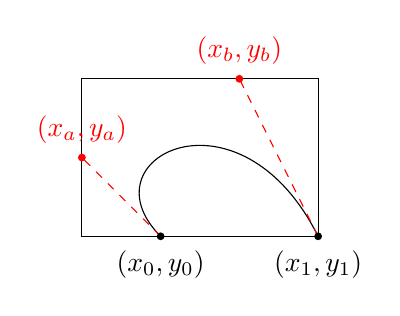
\begin{tikzpicture}[%
	bullet/.style={circle,fill,
		inner sep=1pt}]
 \draw (0,0) .. controls (-1,1) 
 	and (1,2) .. (2,0);
 \draw (current bounding box.south west) 
 	rectangle 
  (current bounding box.north east);
 \draw[red,dashed] 
 	(0,0) -- (-1,1) 
	node[bullet,label=above:{$(x_a,y_a)$}]{}
    (2,0) -- (1,2) 
	node[bullet,label=above:{$(x_b,y_b)$}]{};
 \path (0,0) 
 	node[bullet,label=below:{$(x_0,y_0)$}]{}
 	(2,0) 
	node[bullet,label=below:{$(x_1,y_1)$}]{};
\end{tikzpicture}
\end{codeexample}

As one can see from this illustration, this may lead to drastic overestimates of
the bounding box.

\subsection{Computing the bounding box}

Establishing the precise bounding box has been discussed in various places, the
following discussion uses in part the results from
\url{https://pomax.github.io/bezierinfo/}. What is a cubic Bezier curve? A
cubic Bezier curve running from $(x_0,y_0)$ to $(x_1,y_1)$ with control points
$(x_a,y_a)$ and $(x_b,y_b)$ can be parametrized by
\begin{equation}
 \gamma(t)~=~
 \begin{pmatrix} x(t)\\ y(t) \end{pmatrix}~=~
 \begin{pmatrix}t^3 x_{1}+3 t^2 (1-t) x_{b}+(1-t)^3
   x_{0}+3 t (1-t)^2 x_{a}\\
   t^3 y_{1}+3
   t^2 (1-t) y_{b}+(1-t)^3 y_{0}+3 t (1-t)^2
   y_{a}\end{pmatrix}\;,\label{eq:gammaBezier}
\end{equation}
where $t$ runs from 0 to 1 (and $\gamma(0)=(x_0,y_0)$ and
$\gamma(1)=(x_1,y_1)$). Surely, the bounding box has to contain
$(x_0,y_0)$ and $(x_1,y_1)$. If the functions $x(t)$ and $y(t)$ have extrema in
the interval $[0,1]$, then the bounding box will in general be larger than that.
In order to determine the extrema of the curve, all
we need to find the extrema of the functions $x(t)$ and $y(t)$ for $0\le t\le
1$. That is, we need to find the solutions of the quadratic equations
\begin{equation}
 \frac{\mathrm{d}x}{\mathrm{d}t}(t)~=~0\quad\text{and}\quad
 \frac{\mathrm{d}y}{\mathrm{d}t}(t)~=~0\;.
\end{equation}
% (*parametrization of x:*)
% myx = x0 (1 - t)^3 + 3 xa (1 - t)^2 t + 3 xb (1 - t) t^2 +  x1 t^3 
% (*d1\ne0 condition for t1 and t2 to exist*)
% === (*case d1\ne0*) == 
% d1 =  x0 - x1 - 3 xa + 3 xb
% (*square root, d2=0 \[Rule] only one solution,d2<0 \[Rule] no solution*)
% d2 =  x0*x1 - x1*xa + xa*xa - x0*xb - xa xb +  xb*xb 
% (*first t*)
% t1 = (x0 - 2*xa + xb - sqrt(d2))/(x0 - x1 - 3*xa + 3*xb)
%    = (x0 - 2*xa + xb - sqrt(d2))/d1
% (*second t*)
% t2 = (x0 - 2*xa + xb + sqrt(d2))/(x0 - x1 - 3*xa + 3*xb)
%    = (x0 - 2*xa + xb + sqrt(d2))/d1
% === (*case d1=0*) == 
% (*2nd condition for extra condition: d3\ne0*)
% d3 = x1 + xa - 2 xb
% (*third t*)
% t3 = (x1 + 2*xa -  3*xb)/(2*d3)% d3 = x1 + 3 xa - 3 xb - x0
Let's discuss $x$ first. If the discriminant
\begin{equation}
 d~:=~x_0\,x_1 - x_1\,x_a + x_a\,x_a - x_0\,x_b - x_a x_b +  x_b\,x_b
\end{equation}
is greater than 0, there are two solutions
\begin{equation}
 t_\pm~=~\frac{x_{0}-2x_{a}+x_{b}\pm\sqrt{d}}{%
 	x_{0}-x_{1}-3(x_{a}- x_{b})} \;.
\end{equation}  
If the denominator $x_{0}-x_{1}-3(x_{a}- x_{b})$  vanishes, one may use the
l'Hospital rule to determine the solutions.
In this case, we need to make sure that the bounding box contains, say
$(x(t_-),y_0)$ and $(x(t_+),y_0)$. If $d\le0$, the bounding box does not need to
be increased in the $x$ direction. On the other hand, if there are solutions,
one needs include the points $\bigl(x(t_\pm),y_0\bigr)$ with $x(t)$ from
\eqref{eq:gammaBezier} in the bounding box. 

The analogous statements apply to $y(t)$. 

\subsection{Using the library}

\begin{key}{/pgf/bezier bounding box=\meta{boolean} (default true)}
    Turn the tight bounding box algorithm on and off. The initial value is
	|false|.

	\emph{Caveat:} As can be seen from the derivations, the necessary
	computations involve the squaring of lengths and taking ratios of lengths,
	which can easily lead to |dimension too large| errors. The library uses
	|fpu| to account for that, but errors may still occur.
\end{key}


\begin{codeexample}[width=5cm]
\begin{tikzpicture}[bezier bounding box,%
	bullet/.style={circle,fill,
		inner sep=1pt}]
 \draw (0,0) .. controls (-1,1) 
 	and (1,2) .. (2,0);
 \draw (current bounding box.south west) 
 	rectangle 
  (current bounding box.north east);
 \draw[red,dashed] 
 	(0,0) -- (-1,1) 
	node[bullet,label=above:{$(x_a,y_a)$}]{}
    (2,0) -- (1,2) 
	node[bullet,label=above:{$(x_b,y_b)$}]{};
 \path (0,0) 
 	node[bullet,label=below:{$(x_0,y_0)$}]{}
 	(2,0) 
	node[bullet,label=below:{$(x_1,y_1)$}]{};
\end{tikzpicture}
\end{codeexample}

A few comments are in order. 
\begin{enumerate}
\item For paths with arrow heads one may need to load the
 \texttt{bending} library. This is because otherwise the quick arrow head
 distorts the path, and this happens after the bounding box has been computed.
 Even worse, arrow heads could get deformed.
\item If you shorten a path by some negative length, the bounding box will not
 be accurate either. However, this has nothing to do with curves, it also
 applies to straight lines. So this is not specific to the |bbox| library but
 something that one may want to keep in mind.
\item Let us also note that the computations can lead to |dimension too large| errors.
 These errors do not come directly from the computations done by the library,
 which uses |fpu| for its computations, but from the aftermath. Many of these
 problems can be avoided by using the |fpu| library also for computing
 reciprocals. 
\end{enumerate}

\begin{key}{/pgf/use fpu reciprocal\meta{boolean} (default true)}
  This changes the computation of reciprocals from the standard pgf routine to
  an |fpu| variant. The initial value is |false|.
\end{key}

\endinput


%%% Local Variables:
%%% mode: latex
%%% TeX-master: "pgfmanual-pdftex-version"
%%% End:
